\documentclass[10pt, twocolumn]{article}

\usepackage[utf8]{inputenc}
\usepackage[T2A]{fontenc}
\usepackage[russian]{babel}

\usepackage{indentfirst}
\usepackage{amssymb, amsfonts, amsmath, mathtext}
\usepackage{graphicx}

\usepackage{pgf, tikz}
\usetikzlibrary{arrows}
\definecolor{zzttqq}{rgb}{0.6, 0.2, 0}
\definecolor{qqqqff}{rgb}{0, 0, 1}

\title{Исследование зависимости погрешности численного интегрирования от возмущений в сетке}
\author{Коновалов Андрей, 073}
\date{}

\begin{document}

\maketitle

%\begin{abstract}
%ТУДУ.
%\end{abstract}

\section{Введение}

Рассмотрим определенный интеграл без особенностей
\begin{equation} \label{eq:integral}
  I = \int \limits_a^b f(x) dx.
\end{equation}

Для приближенного вычисления интеграла \eqref{eq:integral} рассмотрим равномерую сетку, то есть разобьем отрезок $[a, b]$ на некоторое число $n$ равных отрезков
\begin{equation} \label{eq:uniform_grid}
  a = x_0 < ... < x_n = b.
\end{equation}

Теперь рассмотрим другую сетку
\begin{equation} \label{eq:bad_grid}
  a = \hat{x}_0 < ... < \hat{x}_n = b,
\end{equation}
равномерную с точностью до некоторой погрешности $\Delta x$. Это означает, что любой узел $\hat{x}_k$ отличается от узла равномерной сетки $x_k$ не более, чем на $\Delta x$, то есть
\begin{equation*}
  |\hat{x}_k - x_k| \leq \Delta x, \;\;\; k = 0, ..., n.
\end{equation*}

Будем считать, что при вычислении значения функции $f(x)$ в некоторой точке $x$ ее значение $f(x)$ известно с некоторой погрешностью $\Delta f$, то есть
\begin{equation*}
  |\hat{f}(x) - f(x)| \leq \Delta f,
\end{equation*}
где $\hat{f}(x)$ - полученное при вычислении значение.

На каждом отрезке $[\hat{x}_k, \hat{x}_{k + 1}]$ построим линейный интерполянт $P_k(x)$ такой, что
\begin{equation*}
  P_k(\hat{x}_k) = \hat{f}(\hat{x}_k), \; P_k(\hat{x}_{k + 1}) = \hat{f}(\hat{x}_{k + 1}).
\end{equation*}

Интеграл интерполянта на $[\hat{x}_k, \hat{x}_{k + 1}]$ будем вычислять по формуле трапеций
\begin{equation*}
  \int \limits_{\hat{x}_k}^{\hat{x}_{k+1}} P_k(x) dx = (\hat{x}_{k + 1} - \hat{x}_k) \cdot \frac{\hat{f}(\hat{x}_{k + 1}) + \hat{f}(\hat{x}_k)}{2}.
\end{equation*}

Рассмотрим функцию $P(x)$, которая на каждом из отрезков $[\hat{x}_k, \hat{x}_{k + 1}]$ совпадает с $P_k(x)$. Искомый интеграл будет вычисляться как
\begin{equation*}
  \hat{I} = \sum \limits_{k = 0}^{n - 1} \int \limits_{\hat{x}_k}^{\hat{x}_{k+1}} P_k(x) dx = \int \limits_a^b P(x) dx
\end{equation*}

В результате, интеграл \eqref{eq:integral} будет вычислен с некоторой погрешностью
\begin{equation} \label{eq:integral_error}
  \Delta I = |\hat{I} - I| = \left| \int \limits_a^b P(x) dx - \int \limits_a^b f(x) dx \right|,
\end{equation}
которая зависит от самой функции $f(x)$, выбранных узлов $\hat{x}_k$ и значений в них $\hat{f}(\hat{x}_k)$.

\section{Теоретическая оценка}

Получим оценку сверху для $\Delta I$, в зависимости от погрешности вычисления значений подынтегральной функции $\Delta f$, а также от погрешности задания узлов сетки $\Delta x$.

Для начала преположим, что выполняется
\begin{equation*}
  h = \frac{b - a}{n} > 2 \Delta x,
\end{equation*}
это понадобится в дальнейшем.

Рассмотрим линейные интерполянты $Q_k(x)$, построенные на узлах равномерной сетки \eqref{eq:uniform_grid}, то есть такие, что
\begin{equation*}
  Q_k(x_k) = f(x_k), \; Q_k(x_{k + 1}) = f(x_{k + 1}),
\end{equation*}
а также функцию $Q(x)$, которая на каждом из отрезков $[x_k, x_{k + 1}]$ совпадает с $Q_k(x)$.

Ясно, что
\begin{equation*}
  \sum \limits_{k = 0}^{n - 1} \int \limits_{\hat{x}_k}^{\hat{x}_{k + 1}} Q_k(x) dx = \int \limits_a^b Q(x) dx
\end{equation*}

Ошибку \eqref{eq:integral_error} оценим как
\begin{equation} \label{eq:i_i1_i2}
  \Delta I \leq \Delta I_1 + \Delta I_2,
\end{equation}
где
\begin{equation*}
  \Delta I_1 = \left| \int \limits_a^b P(x) dx - \int \limits_a^b Q(x) dx \right|
\end{equation*}
\begin{equation*}
  \Delta I_2 = \left| \int \limits_a^b Q(x) dx - \int \limits_a^b f(x) dx \right|
\end{equation*}

Широко известно, что
\begin{equation} \label{eq:i2_error}
  \Delta I_2 \leq \frac{b - a}{8} \sup \limits_{x \in [a, b]} \left| f''(x) \right| h^2,
\end{equation}
где $h = \frac{b - a}{n}$ - шаг равномерной сетки.

Теперь представим $\Delta I_1$ как
\begin{equation*}
  \Delta I_1 = \left| \sum \limits_{k = 0}^{n - 1} \int \limits_{\hat{x}_k}^{\hat{x}_{k + 1}} (P_k(x) - Q_k(x)) dx \right|,
\end{equation*}
и оценим как
\begin{equation} \label{eq:di1}
  \Delta I_1 \leq \sum \limits_{k = 0}^{n - 1} \left| \int \limits_{\hat{x}_k}^{\hat{x}_{k + 1}} (P_k(x) - Q_k(x)) dx \right|.
\end{equation}

Займемся оценкой
\begin{equation} \label{eq:djk}
  \Delta J_k = \left| \int \limits_{\hat{x}_k}^{\hat{x}_{k + 1}} (P_k(x) - Q_k(x)) dx \right|.
\end{equation}

\begin{figure}
\centering

\begin{tikzpicture}[line cap=round, line join=round, >=triangle 45, x=1.0cm, y=1.0cm]
  \clip(1.1, 1.3) rectangle (8.3, 7.7);
  \fill[color=zzttqq, fill=zzttqq, fill opacity=0.1] (2, 4) -- (2, 2) -- (3, 2) -- (3, 4) -- cycle;
  \fill[color=zzttqq, fill=zzttqq, fill opacity=0.1] (6, 5) -- (6, 7) -- (7, 7) -- (7, 5) -- cycle;

  \draw[color=zzttqq] (2, 4) -- (2, 2);
  \draw[color=zzttqq] (2, 2) -- (3, 2);
  \draw[color=zzttqq] (3, 2) -- (3, 4);
  \draw[color=zzttqq] (3, 4) -- (2, 4);
  \draw[color=zzttqq] (6, 5) -- (6, 7);
  \draw[color=zzttqq] (6, 7) -- (7, 7);
  \draw[color=zzttqq] (7, 7) -- (7, 5);
  \draw[color=zzttqq] (7, 5) -- (6, 5);

  \draw[domain=1.1:8.3] plot(\x,{(--4.5--3*\x)/4});
  \draw[domain=1.1:8.3] plot(\x,{(--10--3*\x)/4});

  \draw (3.2, 6.1) node[anchor=north west] {$P_k'(x)$};
  \draw (4.3, 4.5) node[anchor=north west] {$Q_k(x)$};

  \fill[color=qqqqff] (2, 4) circle (1.5pt);
  \draw[color=qqqqff] (1.85, 4.25) node {$A$};
  \fill[color=qqqqff] (2, 2) circle (1.5pt);
  \draw[color=qqqqff] (1.75, 1.90) node {$B$};
  \fill[color=qqqqff] (3, 2) circle (1.5pt);
  \draw[color=qqqqff] (3.20, 1.90) node {$C$};
  \fill[color=qqqqff] (3, 4) circle (1.5pt);
  \draw[color=qqqqff] (3.20, 4.25) node {$D$};

  \draw[color=zzttqq] (1.6, 3.0) node {$2 \Delta f$};
  \draw[color=zzttqq] (3.4, 3.0) node {$2 \Delta f$};
  \draw[color=zzttqq] (2.55, 4.2) node {$2 \Delta x$};
  \draw[color=zzttqq] (2.55, 1.8) node {$2 \Delta x$};

  \fill[color=qqqqff] (6, 5) circle (1.5pt);
  \draw[color=qqqqff] (5.80, 4.80) node {$E$};
  \fill[color=qqqqff] (6, 7) circle (1.5pt);
  \draw[color=qqqqff] (5.85, 7.20) node {$F$};
  \fill[color=qqqqff] (7, 7) circle (1.5pt);
  \draw[color=qqqqff] (7.20, 7.20) node {$G$};
  \fill[color=qqqqff] (7, 5) circle (1.5pt);
  \draw[color=qqqqff] (7.20, 4.80) node {$H$};

  \draw[color=zzttqq] (5.6, 6.0) node {$2 \Delta f$};
  \draw[color=zzttqq] (7.4, 6.0) node {$2 \Delta f$};
  \draw[color=zzttqq] (6.55, 7.2) node {$2 \Delta x$};
  \draw[color=zzttqq] (6.55, 4.8) node {$2 \Delta x$};

  \fill[color=qqqqff] (2.5, 3) circle (1.5pt);
  \draw (2.8, 2.65) node {$(x_k$, $f_k)$};
  \draw[color=qqqqff] (2.5, 3.3) node {$M$};
  
  \fill[color=qqqqff] (6.5, 6) circle (1.5pt);
  \draw (7.2, 5.65) node {$(x_{k + 1}$, $f_{k + 1})$};
  \draw[color=qqqqff] (6.5, 6.3) node {$N$};
\end{tikzpicture}
  
\caption{Интерполянты} \label{fig:interpolation}
\end{figure}

Смысл величины $J_k$ состоит в разнице площадей под прямыми $P_k(x)$ и $Q_k(x)$ на отрезке $[\hat{x}_k, \hat{x}_{k + 1}]$.

На рисунке изображены точки $(x_k, f(x_k))$ и $(x_{k + 1}, f(x_{k + 1}))$, а также их окрестности в виде прямоугольников, в которых лежат точки $(\hat{x}_k, \hat{f}(\hat{x}_k))$ и $(\hat{x}_{k + 1}, \hat{f}(\hat{x}_{k + 1}))$ соответственно.

Заметим, что прямоугольники не пересекаются в силу предположения $x_{k + 1} - x_k = h > 2 \Delta x$.

По определению $Q_k(x)$ - прямая, проходящая через точки $M$ и $N$, а $P_k(x)$ - некоторая прямая, пересекающая оба прямоугольника.

Из рисунка ясно, что разность площадей под прямыми будет максимальна, когда $P_k(x)$ совпадает с $P_k'(x)$, которая проходит через точки $A$ и $F$.
Получим оценку для этой разности.

Запишем уравнения обеих прямых
\begin{equation*}
  Q_k(x) = \frac{x - x_{k + 1}}{x_k - x_{k + 1}} f_k + \frac{x - x_k}{x_{k + 1} - x_k} f_{k + 1},
\end{equation*}
\begin{align*}
  P_k'(x) &= \frac{x - (x_{k + 1} - \Delta x)}{(x_k - \Delta x) - (x_{k + 1} - \Delta x)} (f_k + \Delta f) \; +\\
        &+ \frac{x - (x_k - \Delta x)}{(x_{k + 1} - \Delta x) - (x_k - \Delta x)} (f_{k + 1} + \Delta f),
\end{align*}
где введены обозначения
\begin{equation*}
  f_k = f(x_k), \;\;\; f_{k + 1} = f(x_{k + 1}).
\end{equation*}

Преобразуем $P_k'(x)$:
\begin{align*}
  P_k'(x) &= \frac{x - (x_{k + 1} - \Delta x)}{x_k - x_{k + 1}} (f_k + \Delta f) \; +\\
          &+ \frac{x - (x_k - \Delta x)}{x_{k + 1} - x_k} (f_{k + 1} + \Delta f).
\end{align*}

Оценим величину
\begin{align*}
  \Delta_k = \sup \limits_{x \in [\hat{x}_k, \hat{x}_{k + 1}]} \left| P_k'(x) - Q_k(x) \right|.
\end{align*}

Ясно, что прямые $Q(x)$ и $P_k'(x)$ параллельны, а значит
\begin{align*}
  \Delta_k = \left| P_k'(x_k) - Q_k(x_k) \right|.
\end{align*}

Заметим, что
\begin{equation*}
  Q_k(x_k) = \frac{x_k - x_{k + 1}}{x_k - x_{k + 1}} f_k  = f_k,
\end{equation*}
а
\begin{align*}
  P_k'(x_k) &= \frac{x_k - x_{k + 1} + \Delta x}{x_k - x_{k + 1}} (f_k + \Delta f) \; +\\
            &+ \frac{\Delta x}{x_{k + 1} - x_k} (f_{k + 1} + \Delta f).
\end{align*}

После приведения к общему знаменателю и сокращения некоторых слагаемых, получим
\begin{equation*}
  \Delta_k = \left| \frac{(f_{k + 1} - f_{k}) \Delta x + (x_{k + 1} - x_k) \Delta f}{x_{k + 1} - x_k} \right|.
\end{equation*}

Немного преобразуя, получим:
\begin{equation*}
  \Delta_k = \left| \frac{(f_{k + 1} - f_{k}) \Delta x}{x_{k + 1} - x_k} + \Delta f \right|,
\end{equation*}
а значит справедлива оценка
\begin{equation*}
  \Delta_k \leq \frac{\left| f_{k + 1} - f_{k} \right| \Delta x}{x_{k + 1} - x_k} + \Delta f.
\end{equation*}

Используя, что
\begin{equation*}
  \left| f_{k + 1} - f_{k} \right| \leq \sup \limits_{x \in [x_k, x_{k + 1}]} \left| f'(x) \right| (x_{k + 1} - x_k),
\end{equation*}
получим
\begin{equation*}
  \Delta_k \leq \sup \limits_{x \in [x_k, x_{k + 1}]} \left| f'(x) \right| \Delta x + \Delta f.
\end{equation*}

Обозначим
\begin{equation*}
  \Delta = \sup \limits_{k = 0, ..., n - 1} \Delta_k.
\end{equation*}

Ясно, что
\begin{equation} \label{eq:delta_error}
  \Delta \leq \sup \limits_{x \in [a, b]} \left| f'(x) \right| \Delta x + \Delta f.
\end{equation}

Мы получили оценку для \eqref{eq:djk}:
\begin{equation*}
  \Delta J_k \leq \Delta (\hat{x}_{k + 1} - \hat{x}_k).
\end{equation*}

Эта оценка была получена в предположении, что $f_k \leq f_{k + 1}$. Ясно, что если $f_k > f_{k + 1}$, то прямую $P'_k(x)$ надо проводить через точки $D$ и $G$, но предложенный способ подсчета дает такой же результат и в этом случае.

Возвращаясь к \eqref{eq:di1}, запишем
\begin{equation} \label{i1_error}
  \Delta I_1 \leq \sum \limits_{k = 0}^{n - 1} J_k \leq \Delta (\hat{x}_n - \hat{x}_0) = \Delta (b - a)
\end{equation}

Используя \eqref{eq:i_i1_i2}, \eqref{eq:i2_error}, \eqref{eq:delta_error} и \eqref{i1_error}, получаем, что
\begin{equation*}
  \Delta I \leq \frac{b - a}{8} \sup \limits_{x \in [a, b]} \left| f''(x) \right| h^2 +
\end{equation*}
\begin{equation} \label{result_error}
   + (b - a) (\sup \limits_{x \in [a, b]} \left| f'(x) \right| \Delta x + \Delta f)
\end{equation}

Итого, мы получили оценку сверху для погрешности численного интегрирования \eqref{eq:integral_error} в предположении, что $h > 2 \Delta x$.

\section{Проверка оценки}

В качестве проверки полученной оценки \eqref{result_error} численно посчитаем интеграл от функции
\begin{equation*}
  f(x) = \sin x
\end{equation*}
на интервале $[0, 2 \pi]$ при различных сетках \eqref{eq:bad_grid}.

При этом будем считать, что
\begin{equation*}
  n = 1000, \; \Delta f = 0
\end{equation*}

\begin{figure}
  \centering
  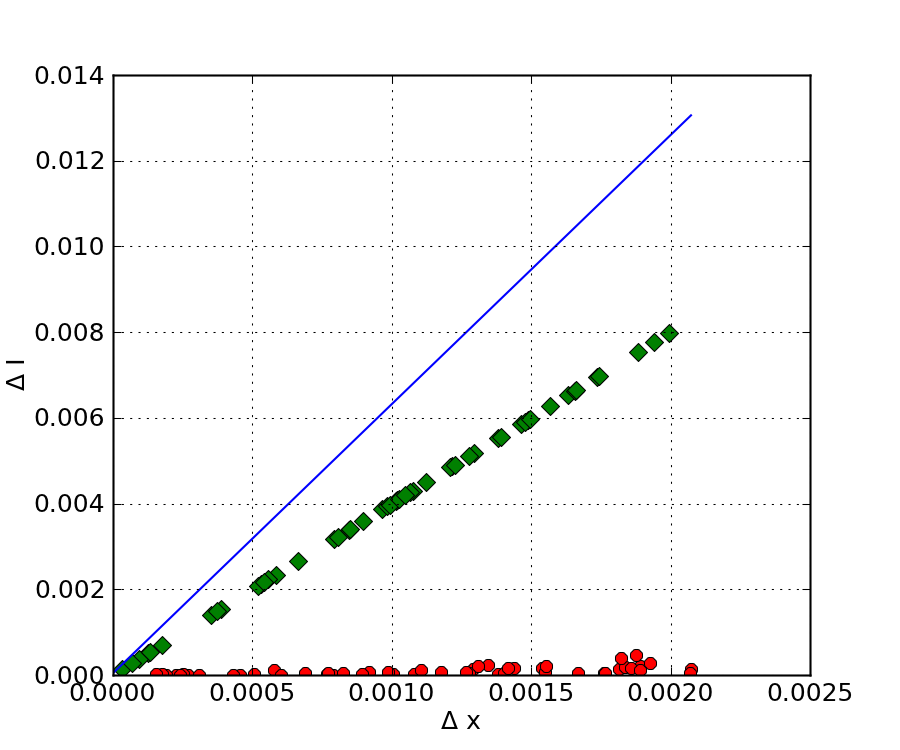
\includegraphics[scale=0.5]{plot.png}
  \caption{Зависимость $\Delta I(\Delta x)$}
\end{figure}

В данном случае $h \approx 0.0063$, а значит $\Delta x$ не может быть больше, чем $\frac{h}{2} \approx 0.0031$.

График зависимости погрешности численного интегрирования $\Delta I$ от погрешности задания узлов сетки $\Delta x$ изображен на рисунке.

Сплошной линии соответствует теоретическая оценка посчитанная по формуле \eqref{result_error}.

Ромбами изображены погрешности численного интегрирование при специально выбираемой 'плохой' сетке.
Выбор точек \eqref{eq:bad_grid} в данном случае осуществлялся таким образом: на интервалах убывания $f(x)$ брались $\hat{x}_k = x_k - \Delta x$, а на интервалах возрастания - $\hat{x}_k = x_k + \Delta x$.

Кругами изображены результаты погрешности при случайно выбираемой сетке. То есть отклонения $\hat{x}_k$ от $x_k$ случайно выбирались из $[-\Delta x, \Delta x]$ с равномерным распределением. Неудивительно, что погрешности получились очень малы, по сравнению с теоретическим максимумом - они просто скомпенсировали друг друга, так как отклонялись равномерно в обе стороны от $x_k$.

\end{document}
